\chapter{Tools}
Developing this kind of systems is extremely complex, but it would be a lot harder without algorithms and libraries made by other people.
In order to make our solution clearer and honor their work, in the following paragraphs I will briefly describe all the tools used by the project.

\section{Language}
Every algorithm is implemented in C++ and all the used libraries bindings are also in the same language due to the fact that the system has to be performance driven. In fact, the QRCode processing should be as fast as possible in order to have the best approximation on location, because the user would be already a few steps ahead of it when the system has finished. However, the proposed solution can be implemented with little modifications in other languages such as Java and Python, but, because we wanted to make the system run in embedded environments with limited resources such as a Beaglebone, C++ is a better fit.
\newline Compiler: \textbf{g++},  version: \textbf{4.7.1}


\section{Developing environment}
A common laptop with the following specifications has been used:
\begin{itemize}
  \item A 2,5 GHz Intel core i7 processor
  \item 8gb of RAM
  \item Integrated graphic card
\end{itemize}
This configuration is more powerful than the one which will be used in a real application. This is due to the fact that the rollator doesn't still have specific requirements but, instead, they are being deducted from experiments on the field. In addition, one of the purpose of the thesis is to proof that using this kind of systems is possible. Therefore, even if the system will not be able to run on a Beaglebone now, in a couple of years it should work without any problem.The chosen operating system is Slackware Linux -current (the current stable version is 14.1). This chose has been only made due to my familiarity with the OS but every GNU/Linux derivate which runs a version of the kernel later than version 2.6.32, because of the camera requirements, will be able to run the necessary software.In fact the system has been tried on Ubuntu Linux 14.04 and openSUSE 13.1 without any problem, in addition the system has been tried on a 2012 Macbook Pro with OSX Mavericks and showed any sign of malfunction. 

\section{The camera}
In order to stream videos or take pictures a Playstation 3 Eye has been used.
This camera can operate at 120Hz with a resolution of 320x240 pixels but we, instead, preferred to operate at 640x480 pixels with a frequency of 60Hz because of the better resolution of the image which grant better working possibilities. The device is automatically recognized and used without issues if the version of the Linux Kernel installed is later than the version 2.6.32, previous versions needs a patch which is available online.
This camera was preferred because of its ability to stream uncompressed video directly \cite{pseyecompr} and for its.


\begin{figure}[hbt]
    \centering
    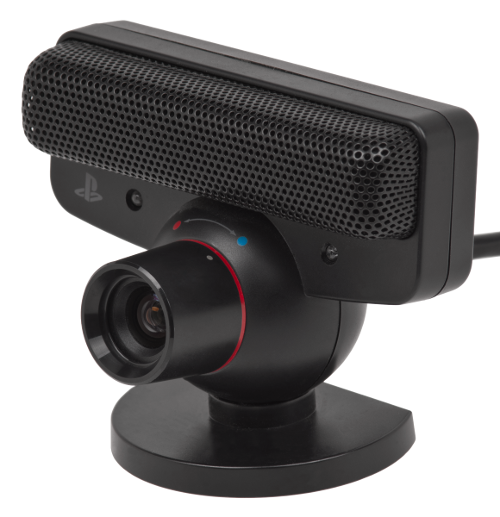
\includegraphics{img/pseye.png}
    \caption{The Playstation Eye}
\end{figure}
 
\newpage
\section{Libraries}

\subsection{OpenCV}
\begin{figure}[hbt]
    \centering
    
\includegraphics[scale=0.5]{img/opencv.png}
    \caption{OpenCV's Logo}
\end{figure}
This library allows image manipulations and processing with consolidated algorithms created by universities and companies.In fact, OpenCV is the de facto standard for computer vision and it is wide-used in many Samsung Cameras, for example, but also on Android smart phones and iOS devices for human faces recognition.However, for our own purposes, the library free us of the burden to communicate with the web cam's hardware by giving APIs to open the streaming channel and taking pictures. In addition it gives us the opportunity to transform a colored image into a greyscale one which helps ZBar's QRCode recognition\footnote{see \textbf{chapter 5} for more information}and provides other methods to save our pictures in different formats and quality . 
\newline Used version: \textbf{2.4.9}

\subsection{ZBar}
\begin{figure}[hbt]
    \centering
    
\includegraphics[scale=0.5]{img/zbar.png}
    \caption{ZBar's Logo}
\end{figure}
The capability of decoding a QRCode is given by the ZBar library, which is open source and can decode also other kind of markers, for example: EAN-13/UPC-A, UPC-E, EAN-8 and Code 128.In addition, it is able to decode from a multitude of sources such as still images, raw intensity sensors and not only from video streams as the project shows. At the core of this possibility there is a streamlined C implementation of the \textbf{ISO/IEC 18004:2000} encoding/decoding standard which is perfect for embedded purposes.
The usage of its API is very simple because it abstracts all the hard work giving an ImageScanner class which returns the list containing all the found symbols. Each symbol is basically a recognized tag which I transform into a class of QRCode with all the necessary data that our system needs such as the center.
\newline Used version: \textbf{0.10}.

\subsection{Eigen}

\begin{figure}[hbt]
    \centering
    
\includegraphics[scale=0.5]{img/eigen.png}
    \caption{Eigen's Logo}
\end{figure}

This library provide abstractions and utilities for linear algebra such as numerical solvers but also matrices and other subject-related algorithms.
It is widely used by big companies such as Google, for its own computer vision and machine learning algorithms.
The whole code is free-software because it is licensed with MPLv2 which guarantees the freedom to choose your own license for the code.It is developed on the flexible C++ templating system which let the developer only use the needed header file. In addition, it has a reasonable compilation time compared to the benefits which brings into the project.\cite{eigeninfo}.
This library is actually used by the rectification algorithm (which is explained below) for its incredible matrix utilities.
\newline Used version: \textbf{3.2.1}.

\section{Algorithms}

\subsection{Rectification}
The rectification process is able to remove perspective and correct distortion from a given picture with rototranslation and the usage of the focal length. The resulting image contains every pixel from the initial photo minus pixels which goes out of bounds. The usage of this algorithm is needed to correct the fact of the web cam which is positioned at a certain height and it is inclined with a certain angle towards the ground\footnote{see \textbf{chapter 5} for more information}. Therefore, any calculation about the center of an already read QRCode would be incorrect without a process which transform the image in a 2D Cartesian plane. In addition, our experiments showed that in certain circumstances the rectification algorithm also aids ZBar to recognize QRCodes\footnote{see the \textbf{results} section for further information}. 








 
